\documentclass[12pt]{article}
\usepackage[margin=1in]{geometry}
\usepackage{amssymb} % math symbols
\setlength{\parskip}{0ex}
\setlength{\parindent}{1em}
%% optional packages -- documentation at ctan.org
\usepackage{graphicx}  % image handline
\usepackage{amsmath}   % enhanced equation environments
\usepackage{tikz}      % block diagrams
\usetikzlibrary{arrows}
\usetikzlibrary{positioning}  % allow relative positioning of tikz elements
\usepackage{pgfplots}  % package for plots, based on tikz
\pgfplotsset{compat=1.18} % set compatibility level
\usepackage{hyperref}


\title{\textbf{Digital Music Synthesizer}}
\author{Hanhee Lee}
\date{December 4, 2024}

\begin{document}
\maketitle
\begin{abstract}
A digital music synthesizer (DMS) is a device that create new waveforms (i.e. sound) using digital signal processing techniques (DSPT) \cite{Wiki}. This paper provides a walk-through of using a DMS to create new waveforms. This includes converting the analog signal to digital using an analog to digital converter (ADC), applying various DSPT to modify the waveform, and converting the processed digital signal to analog using a digital to analog converter (DAC). 
\end{abstract}

\section{Introduction} 
The development of the DMS began in the mid-1900s, changing the way that sound is created and manipulated \cite{AES}. These digital instruments can create an infinite range of sounds, expanding the creative freedom of users in different industries such as gaming, music, movies, etc. In order to understand how the DMS works, it's important to define what a sound is.

\vspace{1em}

A sound is anything that can be heard as a result of vibrations in the air \cite{SS}. To differentiate between sounds, there are three components: 
\begin{enumerate}
    \item \textbf{Amplitude (Loudness):} Corresponds to the height of the waveform.
    \item \textbf{Frequency (Pitch):} Corresponds to the number of cycles that occur in a period.
    \item \textbf{Timbre (Quality):} Corresponds to the number and type of overtones (i.e. harmonics of the fundamental frequency), and their relative strength to one another.
\end{enumerate}

These components can be precisely controlled in the DMS to obtain a desired sound. The DMS process is as follows (see Figure~\ref{fig:process}) \cite{WASIM}:

\begin{enumerate}
    \item \textbf{Digital Oscillator:} Generates digital audio signals using an analog to digital converter, which form the basic waveforms before being synthesized using different DSPT \cite{SS}.

    \item \textbf{Additive Synthesis:} Adding waveforms together to form new sounds \cite{SASP}.
    
    \item \textbf{Modulation} Change various sound parameters using low-frequency oscillators (LFOs), which modulate parameters using slow and periodic signals, and frequency modulation (FM), which modulate the frequency of a carrier waveform using another waveform \cite{MAMO}.
    
    \item \textbf{ADSR Envelope:} The sound are shaped using an envelope generator, which consists of four stages attack, decay, sustain, and release so that it modulates parameters such as amplitude and pitch over time \cite{TTEM}.

    \item \textbf{Filters:} Filters modify the timbre of the waveforms by attenuating or amplifying specific frequency components using subtractive synthesis \cite{TTEM}. Common types include low-pass filters (LPF), high-pass filters (HPF), band-pass filters (BPF), and band-stop filters (BSF).
    
    \item \textbf{Digital to Analog Converter:} Convert the processed digital signal back into an analog format by using the Sampling Theorem to prevent aliasing \cite{SO,FC}. 
\end{enumerate}

Ultimately, sound is processed digitally by converting the signal into the discrete time (DT) system to be processed through the digital music synthesizer before getting converted back into analog format using an ADC. Note, some of the following concepts will be described in the continuous time (CT) domain. However, DMS uses digital sequences, therefore, these DSPT will actually be in DT. It is assumed in this paper that the DSPT will result in samples, $y(nT_s)$, but the specifics will not be discussed.

\begin{figure}[h!]
    \begin{center}
        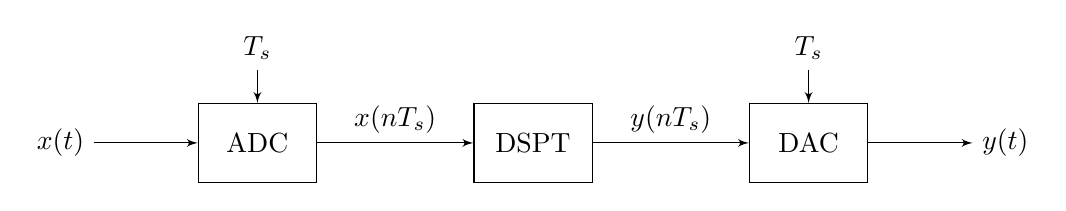
\begin{tikzpicture}[node distance=2cm,auto,>=latex']
    
            % Nodes
            \node [draw, rectangle, minimum width=1.5cm, minimum height=1cm] (CtoD) {ADC};
            \node [right of=CtoD, node distance=3.5cm, draw, rectangle, minimum width=1.5cm, minimum height=1cm] (Filter) {DSPT};
            \node [right of=Filter, node distance=3.5cm, draw, rectangle, minimum width=1.5cm, minimum height=1cm] (DtoC) {DAC};
            
            % Inputs and Outputs
            \node [left of=CtoD, node distance=2.5cm] (input) {$x(t)$};
            \node [right of=DtoC, node distance=2.5cm] (output) {$y(t)$};
            
            % Connections
            \draw [->] (input) -- (CtoD) node[midway, above] {};
            \draw [->] (CtoD) -- (Filter) node[midway, above] {$x(nT_s)$};
            \draw [->] (Filter) -- (DtoC) node[midway, above] {$y(nT_s)$};
            \draw [->] (DtoC) -- (output) node[midway, above] {};
            
            % Sampling Period Annotations
            \node [above of=CtoD, node distance=1.2cm] (Ts1) {$T_s$};
            \node [above of=DtoC, node distance=1.2cm] (Ts2) {$T_s$};
            \draw [->] (Ts1) -- (CtoD);
            \draw [->] (Ts2) -- (DtoC);
        
        \end{tikzpicture}
    \end{center}
    \caption{Block diagram of the DMS process \cite{SO}.}
    \label{fig:process}
\end{figure}

\section{Digital Oscillator}
The DMS uses a digital oscillator to replicate any musical instruments in the $20 [\text{Hz}]$ to $20000 [\text{Hz}]$ range (i.e. human hearing range) \cite{SS}. Specifically, a typical type of digital oscillator is a wave-table oscillator, which performs the wave table lookup operation consisting of two steps \cite{TTEM}:
\begin{enumerate}
    \item Pre-compute digital audio signals, $x[n]$, consisting of a sequence of samples $n=0,1,\ldots,N-1$, where $N$ is the length of the sequence. For periodic waveforms, the $N$ samples of any desired waveform can be precomputed using the Fourier series.
    \item Produce an output $z[n]=x[y[n]]$ such that the input signal $y[n]$ is the index to get the specific values from $x[n]$.
\end{enumerate}

\subsection{Sampling}
While the wave table oscillator is effective for generating a range of periodic waveforms, its limited by having to know what the analytical form of the waveform is before pre-computing the digital audio signals. As a result, to ensure that the DMS can receive any sound (e.g. instruments, sound effects, etc), sampling can be used. Sampling is a process that involves recording a live audio signal into a wave table (i.e. digital sequence) \cite{TTEM}. These samples will accumulate in the DMS' memory as a stream of numbers, which can then be further processed using DSPT \cite{SS}.
\vspace{1em}

To ensure that there is no loss of information from turning the analog signal into a digital signal, the conversion process must follow the Sampling theorem \cite{Sampling_Theorem, FC}:
\vspace{1em}

Let the continuous-time signal \( x(t) \) be band-limited, i.e., the Fourier transform \( X(f) \) satisfies:
\begin{equation}
    X(f) = 0 \quad \text{for } |f| > f_{\text{max}}.
\end{equation}

Then $x(t)$ can be fully recovered by sampling in intervals of $T_s$ (sampling period), if $x(t)$ is sampled at the Nyquist rate:
\begin{equation}
    f_s > 2 f_{\text{max}}
\end{equation}

\begin{itemize}
    \item \( f_s \): Sampling frequency.
    \item \( f_{\text{max}} \): Maximum frequency of the original continuous-time signal.
\end{itemize}

It is a reasonable assumption to have $x(t)$ be bandlimited due to the audio signals being heard between $20 [\text{Hz}]$ to $20000 [\text{Hz}]$ range for a human. As a result, live waveforms can be sampled at a rate of $f_s$ such that 
$$\{\ldots,x(-2T_s),x(-T_s),x(0),x(T_s),x(2T_s),\ldots\},$$
which will stay ensure that the signal can be reconstructed later on \cite{FC}. The Nyquist rate ensures that aliasing doesn't occur where the sampling frequency \( f_s < 2 f_{\max} \), which would distort the original signal, making it impossible to reconstruct the signal \cite{Sampling_Theorem}. Even though the minimum requirement is at least $2f_{\max}$, DMS will over sample to the standard audio sample rate of $44.1 \text{[kHz]}$ or higher \cite{AB}. This enables the user to have greater creative freedom in terms of synthesizing the audio for different purposes without losing information in the signal. 
\vspace{1em}

In order to convert these signals into a digital sequence, the following process is used (see Figure~\ref{fig:1}). Firstly, $x(t)$ is sampled at a rate significantly higher than the Nyquist rate (oversampling), which have a continuous range of possible amplitudes \cite{SO}. As a result, a quantizer is used to map these continuous amplitudes to a discrete set of amplitudes with quantization interval $\Delta$ to produce $\hat{x} (nT_s)$. Finally, the quantized signal is passed into an encoder, which produces a digital sequence for further processing in the DMS.

\begin{figure}[h!]
    \begin{center} % Center the diagram on the page
    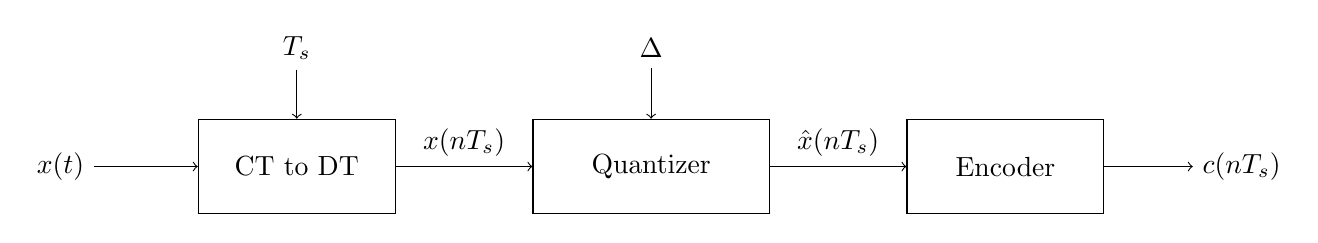
\begin{tikzpicture}[node distance=4.5cm, auto] % Increased node distance for more spacing
    
        % Nodes
        \node [draw, rectangle, minimum width=2.5cm, minimum height=1.2cm] (CD) {CT to DT};
        \node [right of=CD, draw, rectangle, minimum width=3cm, minimum height=1.2cm] (Quantizer) {Quantizer};
        \node [right of=Quantizer, draw, rectangle, minimum width=2.5cm, minimum height=1.2cm] (Encoder) {Encoder};
    
        % Inputs and Outputs
        \node [left of=CD, node distance=3cm] (input) {$x(t)$}; % Continuous-time Input
        \node [right of=Encoder, node distance=3cm] (output) {$c(nT_s)$}; % Encoded Output
    
        % Intermediate Signals
        \node [above of=CD, node distance=1.5cm] (Ts) {$T_s$}; % Sampling period
        \node [above of=Quantizer, node distance=1.5cm] (Delta) {$\Delta$}; % Quantization step size
    
        % Connections (Arrows)
        \draw [->] (input) -- (CD); % From input to C/D
        \draw [->] (CD) -- (Quantizer) node[midway, above] {$x(nT_s)$}; % From C/D to Quantizer
        \draw [->] (Quantizer) -- (Encoder) node[midway, above] {$\hat{x}(nT_s)$}; % From Quantizer to Encoder
        \draw [->] (Encoder) -- (output); % From Encoder to Output
    
        % Additional Arrows
        \draw [->] (Ts) -- (CD); % Sampling period to C/D
        \draw [->] (Delta) -- (Quantizer); % Quantization step size to Quantizer
    
    \end{tikzpicture}
    \end{center}
    \caption{Block diagram of the ADC \cite{SO}.}
    \label{fig:1}
\end{figure}
\newpage

\section{Additive Synthesis}
Additive synthesis takes advantage of the fact that any sound can be expressed as a sum of sinusoids \cite{SASP}. Specifically, by summing over $N$ sinusoidal components, the user can modulate these components by relatively slowly varying amplitude and frequency envelopes. The equation for additive synthesis is:
\begin{equation}
    y(t) = \sum_{i=1}^{N} A_i(t) \sin\left(\theta_i (t)\right)
\end{equation}
\begin{itemize}
    \item $A_i(t) \in \mathbb{R}$: Amplitude of $i$th partial over time $t$
    \item $\theta_i (t) = \int_0^t \omega_i(t)dt + \phi_i(0) \in \mathbb{R}$
    \begin{itemize}
        \item $\omega_i(t)=\frac{d\theta_i(t)}{dt} \in \mathbb{R}$: Radian frequency of $i$th partial vs. time.
        \item $\phi_i(0) \in \mathbb{R}$: Phase offset of $i$th partial at time $0$.
    \end{itemize}
\end{itemize}

As a result, by controlling these parameters, additive synthesis provides a means to generate sounds by assigning each sinusoid a separate envelope that can control the development of timbre and loudness with time \cite{MAMO}. 

\section{Modulation}
Modulation enables variations in loudness, pitch, and timbre. Two common techniques is using LFOs and FM. 

\subsection{Low-Frequency Oscillator}
An LFO is a signal generator that produces slow, periodic waveforms, typically within the range of $0.1 [\text{Hz}]$ to $20 [\text{Hz}]$ (i.e. below human human hearing levels) \cite{MAMO}. The purpose of an LFO is not to generate sound directly, but to modulate various parameters of a waveform periodically. There are many parameters that the LFO can affect \cite{EDMPROD}:
\begin{enumerate}
    \item \textbf{Waveform:} The shape of the oscillation that the LFO generates (e.g. sine, triangle, square, and sawtooth).
    \item \textbf{Frequency:} The speed of the modulation, where a low frequency will cause slow changes, while a high frequency will create rapid changes. 
    \item \textbf{Depth:} Controls the extent of the modulation's influence on the parameter of interest.
    \item \textbf{Mode:} Determines how the LFO's cycle behaves during playback. In trigger mode, the LFO restarts its waveform cycle every time a new signal is played. In envelope mode, the LFO acts as an envelope (completing the period and stopping once the waveform reaches its end). 
\end{enumerate}

With these parameters defined, we can now examine how they apply to the most common waveform shapes. The following variables will be used to describe the most common waveforms in CT:
\begin{itemize}
    \item \( A \): Amplitude of the waveform, determining its loudness.
    \item \( f \; [\text{Hz}]\): Frequency of the waveform, determining its pitch. 
    \item \( t \; [s]\): Time.
    \item \( \phi \; [\text{rad}]\): Phase offset.
    \item \( n \): Harmonic number, corresponding to integer multiples of the fundamental frequency.
    \item \( T \): Period of the waveform.
\end{itemize}

Each of these waveforms offers unique characteristics that influence the modulation that can be produced by the LFO \cite{SSTS}:
\begin{enumerate}
    \item \textbf{Sine Wave:} The sine wave contains only the fundamental frequency with no partial tones, represented as:
    \begin{equation}
        x(t) = A \sin(2\pi f t + \phi)
    \end{equation}
    The sine wave sounds like a pure tone due to only having one frequency, which can be used to create every other waveform. 

    \item \textbf{Square Wave:} The square wave comprises a fundamental frequency and its odd harmonics, represented as \cite{SW}:
    \begin{equation}
        x(t) = \frac{4}{\pi} \sum_{n=1,3,5,\ldots}^\infty \frac{1}{n} \sin\left(\frac{n \pi t}{L}\right)
    \end{equation}
    The square wave sounds richer and buzzier, which is more harsher than the sine wave \cite{SSTS, OTTO}. The sharp transitions between high and low values give the square wave a characteristic "on-off" sound.

    \item \textbf{Sawtooth Wave:} The sawtooth wave contains a fundamental frequency and all harmonics of the fundamental, represented as \cite{STW}:
    \begin{equation}
        x(t) = \frac{1}{2} - \frac{1}{\pi} \sum_{n=1}^\infty \frac{1}{n} \sin\left(\frac{n \pi t}{L}\right)
    \end{equation}
    The sawtooth wave is the buzziest and richest in terms of harmonics \cite{OTTO}.

    \item \textbf{Triangle Wave:} The triangle wave contains a fundamental frequency and its odd harmonics, represented as \cite{TW}:
    \begin{equation}
            x(t) = \sum_{k=1,3,5\ldots}^{\infty} \frac{8A}{\pi^2 k^2} (-1)^{(k-1)/2} \cos\left( 2 \pi \frac{k}{T} t \right)
    \end{equation}
    The triangle wave has a harsher sound than sine waves, but a softer sound than square waves \cite{OTTO}.
\end{enumerate}
As a result, LFOs have many applications to create different effects. Two main effects are
\begin{enumerate} 
    \item \textbf{Vibrato Effect:} Modulates the pitch of a waveform by periodically varying the pitch using an LFO, in which the intensity is determined by the amplitude, and the frequency determines the speed of the fluctuations \cite{CC}.

    \item \textbf{Tremelo Effect:} Modulates the amplitude of a waveform by changing the volume of the signal periodically, which are usually made with sine or triangle waveforms \cite{CC1}.
\end{enumerate}

\subsection{Frequency Modulation}
The Yamaha DX7 was invented by John Chowning in 1983, which was the first commercially available DMS that used FM synthesis \cite{MAMO}. In order to understand how FM synthesis works, we will use the Yamaha DX7's methodology of computing FM. Specifically, FM synthesis modulates the frequency of a carrier waveform using a modulating waveform inside the argument. The frequency modulated signal can be represented as 
\begin{equation}
    \sin(\omega_c t + I \sin \omega_m t)
\end{equation}
\begin{itemize}
    \item \( \omega_c = 2\pi f_c \): Carrier angular frequency.
    \item \( \omega_m = 2\pi f_m \): Modulating angular frequency.
    \item \( I \): Modulation index, which can determine the extent of frequency deviation $d$ as $d=If_m$
\end{itemize}
where the values are calculated using digital lookup tables for the function \cite{MAMO}.
\vspace{1em}

Furthermore, the FM synthesis equation can be represented in terms of its Fourier Series using the Bessel functions $J_n(I)$:
    \begin{equation}
        \sin(\omega_c t + I \sin \omega_m t) = \sum_{n=-\infty}^\infty J_n(I) \sin(\omega_c + n\omega_m)t
    \end{equation}
where $J_n(I)$ represents the amplitude of the $n$th sideband \cite{MAMO}. The Yamaha DX7 implements this Fourier series using two operators:
\begin{enumerate}
    \item \textbf{Operator 1:} Generates the carrier signal, whose amplitude envelope dictates how the final signal's amplitude changes over time \cite{MAMO}. 
    \item \textbf{Operator 2:} Produces the modulating signal, and its amplitude envelope controls the modulation index $I$, which influences the harmonic content of operator 1's output using the frequency deviation \cite{MAMO}. 
\end{enumerate}

For small values of $I$, the frequency spectrum is dominated by $\omega_c$, resulting in a pure sine wave \cite{MAMO}. As $I$ increases, the frequency spectrum has more harmonic components, with higher-order sidebands contributing more significantly. Consequently, operator 1 defines the amplitude of the final output signal, while operator 2 shapes the timbre by controlling the modulation index $I$. As a result, FM synthesis can create sounds such as bell timbres, metallic tones, tine tones of electric pianos, punchy bass, and synthetic brass sounds \cite{OL}.

\section{ADSR Envelope}

The ADSR (attack, decay, sustain, and release) envelope generator (EG) produces an audio signal that rises and falls smoothly, controlling the loudness of the sound \cite{TTEM}. The four stages of the ADSR envelope are as follows (see Figure~\ref{fig:adsr}) \cite{MAMO}:
\begin{enumerate}
    \item \textbf{Attack:} Time it takes for the initial rise to the maximum amplitude when the envelope is triggered on. 
    \item \textbf{Decay:} Time it takes for the transition from its maximum amplitude to the sustain amplitude level.
    \item \textbf{Sustain:} The level at which the sound is held at steady state.
    \item \textbf{Release:} The time it takes for the sound to go to 0 amplitude after the note is released. 
\end{enumerate}

\begin{figure}[h!]
    \centering
    \begin{tikzpicture}[scale=1]
        % Axes
        \draw[->] (0, 0) -- (6, 0) node[anchor=north] {Time};
        \draw[->] (0, 0) -- (0, 4) node[anchor=east] {Amplitude};

        % ADSR curve
        \draw[thick,blue] (0, 0) -- (1, 3) -- (2, 2) -- (4, 2) -- (5, 0);

        % Labels
        \node[anchor=north] at (1, 0) {A};
        \node[anchor=north] at (2, 0) {D};
        \node[anchor=north] at (4, 0) {S};
        \node[anchor=north] at (5, 0) {R};
    \end{tikzpicture}
    \caption{ADSR envelope applied to a sound signal \cite{MAMO}.}
    \label{fig:adsr}
\end{figure}

The ADSR envelope is activated by a trigger control stream that turns the envelope on and off \cite{TTEM}. When the generator is triggered on, the envelope goes through the attack, decay, and sustain segments, while triggering it off causes it to start the release segment. 
\vspace{1em}

The ADSR EG has 5 main parameters \cite{TTEM}. Firstly, the level parameter determines the envelope's maximum amplitude. Secondly, the attack and decay parameters set the duration of these segments, respectively. Thirdly, the sustain parameter specifies the amplitude at which the sound is held during the sustain segment. Fourthly, the release parameter controls the duration of the release segment. Together, these parameters, along with the timing of the on and off triggers can determine the ADSR envelope's output. 
\vspace{1em}

As a result, the ADSR EG can control the amplitude, tones, and timbre of the sound \cite{TTEM}. Some examples include \cite{MC}: 
\begin{itemize}
    \item \textbf{Rich, lush tones:} Long attack, long release. 
    \item \textbf{Percussive, staccato sounds:} Short attack, short release. 
    \item \textbf{Snares or Hi-hats Instruments:} Long release time.
    \item \textbf{Focus on peaks:} Short sustain, long decay.
\end{itemize}

\section{Subtractive Synthesis}
Subtractive synthesis uses filters to shape the spectral envelope of a sound \cite{TTEM}. Specifically, the resulting sound is the product of the envelope of the original sound with the frequency response of the filter. Starting from a waveform, the user can removes specific frequency components using filters to shape the final sound signal. The process can be represented in the frequency domain as:
\begin{equation}
    Y(f) = X(f) H(f)
\end{equation}
\begin{itemize}
    \item \( X(f): \) Frequency response of the original sound.
    \item \( H(f): \) Frequency response of filter.
    \item \( Y(f): \) Frequency response of the output signal.
\end{itemize}

By manipulating the harmonic content of waveforms, filters significantly influence the brightness of the sound \cite{MAMO}. The operation of a filter is typically described in terms of \cite{TTEM}:
\begin{enumerate}
    \item \textbf{Pass-band:} The range of frequencies that the filter allows to pass with minimal attenuation.
    \item \textbf{Stop-band:} The range of frequencies that the filter attenuates significantly.
    \item \textbf{Transition-band:} Due to physical limitations, ideal filters with an abrupt transition are not realizable in practical implementations. Therefore, the transition band denotes the intermediate region between the pass-band and stop-band. 
\end{enumerate}

\subsection{Types of Filters}
In the DMS, four main filter types are used: low-pass, high-pass, band-pass, and band-stop filters. Each type has a specific role in subtractive synthesis, and their functionality is described below with the following variables:
\begin{itemize}
    \item $H(f)$: Frequency response of the filter.
    \item \(f_c\): Center frequency of the pass-band.
    \item \(W\): Bandwidth of the pass-band.
\end{itemize}

\begin{enumerate}
    \item \textbf{LPF:} Allows low frequency components to pass through while attenuating higher frequencies above a cutoff frequency \(f_c\) \cite{TTEM}. The ideal frequency response of an LPF is expressed as:
\begin{equation}
    H(f) = 
    \begin{cases} 
    1 & \text{if } |f| \leq f_c, \\
    0 & \text{if } |f| > f_c.
    \end{cases}
\end{equation}

\item \textbf{HPF:} Allows high-frequency components to pass through while attenuating frequencies below a specified cutoff \(f_c\) \cite{TTEM}. The ideal frequency response of an HPF is:
\begin{equation}
    H(f) = 
    \begin{cases} 
    1 & \text{if } |f| > f_c, \\
    0 & \text{if } |f| \leq f_c.
    \end{cases}
\end{equation}

\item \textbf{BPF:} Allows frequencies within a specified range, or \textit{bandwidth}, to pass through while attenuating frequencies outside this range \cite{TTEM}. Band-pass filters are useful for emphasizing specific harmonics or resonances. The ideal frequency response is:
\begin{equation}
    H(f) = 
    \begin{cases} 
    1 & \text{if } |f| \leq f_c + W, \\
    0 & \text{otherwise}.
    \end{cases}
\end{equation}

\item \textbf{BSF:} Attenuates frequencies within a specified range (notch) while allowing frequencies outside this range to pass through \cite{TTEM}. The ideal frequency response is:
\begin{equation}
    H(f) = 
    \begin{cases} 
    1 & \text{if } |f| \geq f_c + W, \\
    0 & \text{otherwise}.
    \end{cases}
\end{equation}
\end{enumerate}

\section{Digital to Analog Conversion}
DAC is the process of converting a DT signal into a CT signal so that analog devices (e.g. speakers, headphones, etc) can play the sound. 
\vspace{1em}

The DAC process (see Figure~\ref{fig:DAC}) involves two steps. First, interpolating the samples after applying DSPT
$$\{\ldots,y(-2T_s),y(-T_s),y(0),y(T_s),y(2T_s),\ldots\}$$
to fully reconstruct a synthesized CT signal without loss of information \cite{SO,FC}. This can also be represented mathematically by multiplying the samples by an impulse train, along with its corresponding Fourier transform using the sifting property as: 
\begin{equation}
    y_s(t) = \sum_{n \in \mathbb{Z}} y(nT_s) \delta(t - nT_s) \overset{\mathcal{F}}{\leftrightarrow} \frac{1}{T_s} \sum_{k \in \mathbb{Z}} Y \left(f - \frac{k}{T_s}\right)
\end{equation}

\vspace{1em}

Second, in an ideal situation, the samples are passed through an ideal LPF, which removes the frequency components. The ideal LPF $h(t)$ and its Fourier transform $H(f)$ is:
\begin{equation}
    h(t) = \text{sinc} \left(\frac{t}{T_s} \right)H(f) = T_s \text{rect} (fT_s) 
\end{equation}

This LPF will remove all frequencies above the cutoff frequency $\frac{f_s}{2}$ to ensure that the only frequencies that remain are associated with the synthesized CT signal $y(t)$ (i.e. within the Nyquist range \( |f| \leq \frac{f_s}{2} \)) \cite{SO}. In the time domain, the fully reconstructed CT signal $y(t)$ is 
\begin{equation}
    y(t) = \sum_{n \in Z} y(nT_s) \text{sinc} \left(\frac{t-nT_s}{T_s}\right)
\end{equation}

\begin{figure}[h!]
    \begin{center} % Center the diagram on the page
        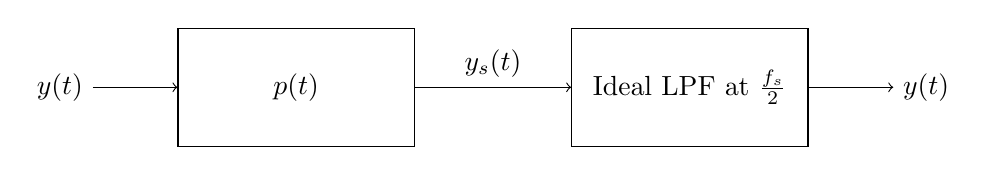
\begin{tikzpicture}[node distance=5cm, auto] % Increased node distance for spreading out
        
            % Nodes
            \node [draw, rectangle, minimum width=3.0cm, minimum height=1.5cm] (Impulse) {$p(t)$};
            \node [right of=Impulse, draw, rectangle, minimum width=3.0cm, minimum height=1.5cm] (Filter) {Ideal LPF at $\frac{f_s}{2}$};
        
            % Inputs and Outputs
            \node [left of=Impulse, node distance=3cm] (input) {$y(t)$}; % Discrete-time Input
            \node [right of=Filter, node distance=3cm] (output) {$y(t)$}; % Continuous-time Output
        
            % Connections (Arrows)
            \draw [->] (input) -- (Impulse) node[midway, above] {};
            \draw [->] (Impulse) -- (Filter) node[midway, above] {$y_s(t)$};
            \draw [->] (Filter) -- (output);
        
        \end{tikzpicture}
    \end{center}
    \caption{Block diagram of the DAC \cite{SO}.}
    \label{fig:DAC}
\end{figure}

Realistically, many DAC use a zero-order hold for the reconstruction filter, which produces a staircase approximation to the original signal $y(t)$ \cite{SO}. The process shown above with the ideal LPF is the same, but with the filter now being \cite{FC}: 
\begin{equation}
    H(f) = e^{-j 2\pi f \frac{T_s}{2}} \cdot T_s \text{sinc}(fT_s)
\end{equation}

\section{Conclusion}
Ultimately, this paper presented an overview of the DMS. Using a digital oscillator, analog signal are converted to a digital form via an ADC. The resulting digital signal can then be modified through many DSPT such as additive synthesis, LFOs, FM, ADSR envelop generators, and subtractive synthesis. Finally, after modifying the digital waveform, it can be converted back to an analog form using a DAC.
\vspace{1em}

For readers interested in further exploration of the DMS, please read the \textit{The Theory and Technique of Electronic Music} \cite{TTEM}, \textit{Music: A Mathematical Offering} (Chapters 7 and 8) \cite{MAMO}, and \textit{Spectral Audio Signal Processing} \cite{SASP}, along with the references therein. 
\newpage
\begin{thebibliography}{99}  %% Organized alphabetically by author OR
                            %% in order of citation
                            %% Increase to 99 if you have more than 9 refs
\bibitem{Wiki} “Digital synthesizer,” Wikipedia, \href{https://en.wikipedia.org/wiki/Digital_synthesizer}{Link}
\bibitem{AES} History and practice of Digital Sound Synthesis, \href{https://www.aes.org/technical/heyser/downloads/AES121heyser-Smith.pdf}{Link} 

\bibitem{SS}
H. Massey, “Subtractive 101, part one: The basics,” Synth,  \href{https://yamahasynth.com/learn/synth-programming/subtractive-synthesis-101-part-one-the-basics}{Link}.

\bibitem{WASIM} “Auto-tune - the best vocal plug-ins available,” Auto-Tune - The Best Vocal Plug-Ins Available, \href{https://www.antarestech.com/community/what-are-synths-in-music}{Link}

\bibitem{SASP} “Spectral Audio Signal Processing,” CCRMA, \href{https://ccrma.stanford.edu/~jos/sasp/}{Link}

\bibitem{MAMO} Music: A mathematical offering Dave Benson, \href{https://logosfoundation.org/kursus/music_math.pdf}{Link}

\bibitem{TTEM} The theory and technique of electronic music, \href{http://msp.ucsd.edu/techniques/v0.09/book.pdf}{Link}

\bibitem{SO} Schaum’s outlines of digital signal processing, \href{https://courses.e-ce.uth.gr/CE446/schaum.pdf}{Link} 

\bibitem{FC} F. R. Kschischang, "Notes on the Sampling Theorem"

\bibitem{Sampling_Theorem} GeeksforGeeks, “Nyquist sampling theorem - statement, working, aliasing, applications,” GeeksforGeeks, \href{https://www.geeksforgeeks.org/nyquist-sampling-theorem/}{Link}

\bibitem{AB} Sample rates and audio sampling: A guide for beginners | adobe, \href{https://www.adobe.com/uk/creativecloud/video/discover/audio-sampling.html}{Link}

\bibitem{EDMPROD} S. Haven, “LFO like a Boss: The Complete Beginner’s Guide for 2024,” EDMProd, \href{https://www.edmprod.com/lfo/}{Link} 

\bibitem{SSTS} N. Robehmed, “Sine, square, Triangle, saw,” Perfect Circuit, \href{https://www.perfectcircuit.com/signal/difference-between-waveforms?srsltid=AfmBOoqnJ4EZmI1aorjWtuXuEAHn448bQlZGz2gpxDJSVu2E_FpVeH2Y}{Link}

\bibitem{SW} “Fourier series--Square Wave,” from Wolfram MathWorld, \href{https://mathworld.wolfram.com/FourierSeriesSquareWave.html}{Link}

\bibitem{OTTO} R. Smith, “The basic waveforms in synthesis - on the track,” On The Track - Music theory, beats, and more, \href{https://onthetrackofficial.com/the-basic-waveforms-in-synthesis/}{Link}

\bibitem{STW} “Fourier series--sawtooth wave,” from Wolfram MathWorld, \href{https://mathworld.wolfram.com/FourierSeriesSawtoothWave.html}{Link}

\bibitem{TW} “Fourier series--Triangle Wave,” from Wolfram MathWorld, \href{https://mathworld.wolfram.com/FourierSeriesTriangleWave.html}{Link} 

\bibitem{CC} Complete guide the vibrato audio modulation effect - fox music production, \href{https://foxmusicproduction.com/vibrato-audio-modulation-effect/}{Link}

\bibitem{CC1} K. Pearsall, “Effects guide: Get to know tremolo,” What is Tremolo?, \href{https://www.fender.com/articles/parts-and-accessories/pedal-board-primer-get-to-know-tremolo#:~:text=Tremolo%20is%20a%20modulation%20effect%20that%20rhythmically%20changes%20the%20volume,the%20signal%20up%20and%20down.}{Link}

\bibitem{OL} “Frequency modulation (FM) synthesis,” Apple Support, \href{https://support.apple.com/en-ca/guide/logicpro/lgsife418213/mac#:~:text=FM%20synthesis%20is%20extremely%20good,bass%20and%20synthetic%20brass%20sounds.}{Link}

\bibitem{MC} “ADSR envelopes explained: 4 stages of an ADSR envelope - 2024,” MasterClass, \href{https://www.masterclass.com/articles/adsr-envelope-explained#4bPVgIZ4W9GAOAyN3yNHDN}{Link} 

\end{thebibliography}

\end{document}
